\section{Usecase diagram và đặc tả use-case}
        \subsection{Usecase hệ thống}
            \begin{figure}[H]
                \centering
                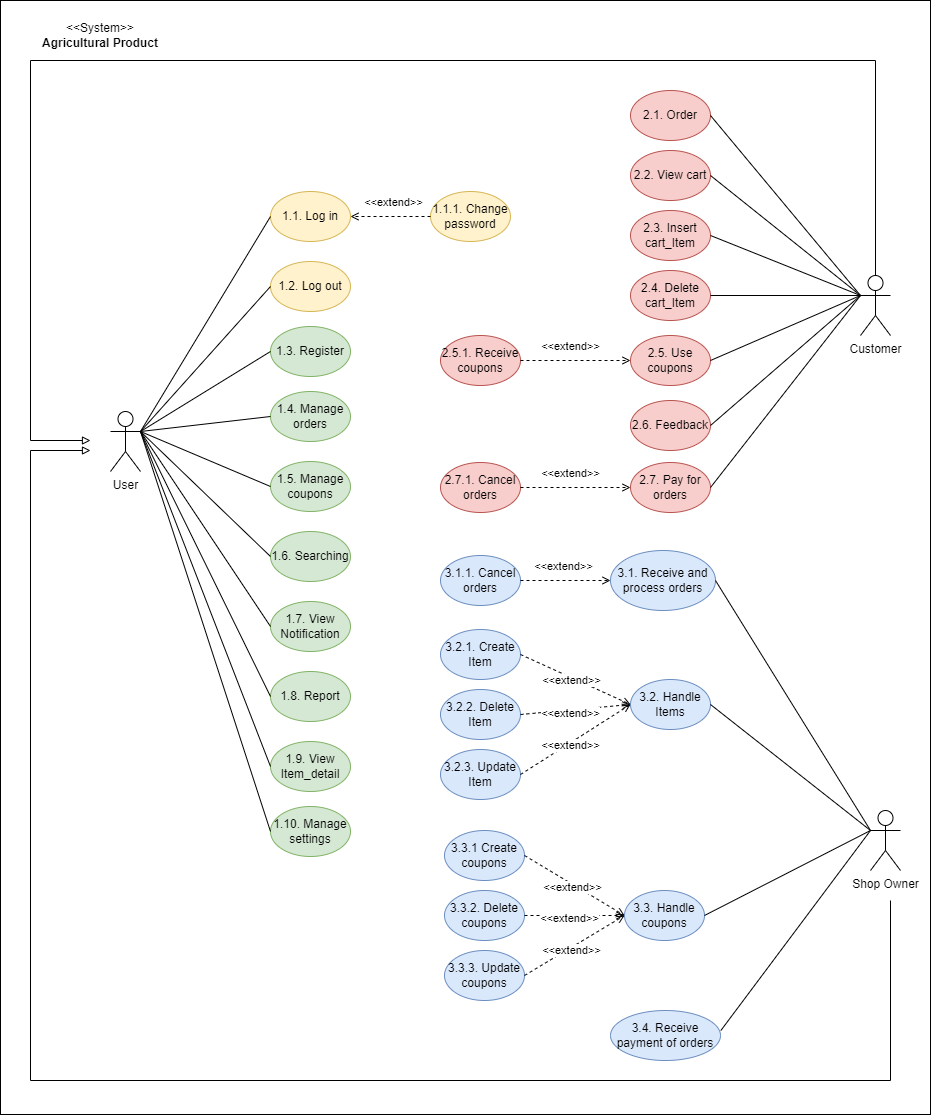
\includegraphics[width=1\linewidth]{Images/usecase.png}
                \vspace{1em}
                \caption{Use-case hệ thống}
            \end{figure}
        \newpage
        \subsection{Đặc tả usecase}
            \subsubsection{Đăng nhập}
            \begin{usecase_table}[Use case Đăng nhập]
                    \hline
                    Use Case ID & UC-1.1 \\
                    \hline
                    Use Case Name & Log in \\
                    \hline
                    Actor(s) & Khách hàng, chủ cửa hàng\\
                    \hline
                    Description & Đăng nhập vào hệ thống\\
                    \hline
                    Priority & Cao \\
                    \hline
                    Trigger & Người dùng muốn đăng nhập vào hệ thống \\
                    \hline
                    Pre-Conditions & Tài khoản người dùng đã được tạo sẵn.
                    \newline
                    1. Tài khoản người dùng đã được phân quyền.
                    \newline
                    2. Thiết bị của người dùng đã được kết nối internet.\\
                    \hline
                    Post-Conditions & Người dùng đăng nhập hệ thống thành công.
                    \newline
                    Hệ thống ghi nhận đăng nhập thành công vào Activity Log.\\
                    \hline
                    Basic flow &   
                            1. Hệ thống hiển thị giao diện đăng nhập \newline
                    	2. Người dùng nhập thông tin đăng nhập vào các trường tương ứng trên giao diện và chọn nút đăng nhập\newline
                    	3. Hệ thống kiểm tra thông tin đăng nhập \newline
                    	4. Hệ thống thông báo đăng nhập thành công \newline
                    	5. Hệ thống hiển thị giao diện màn hình chính \\
                    \hline
                    Alternative flow  & Alternative 2.1-1: tại bước 2 \newline
                        	2a. Người dùng chọn phương thức đăng nhập bằng tài khoản của bên thứ ba \newline
                                2a1. Hệ thống chuyển sang màn hình đăng nhập của bên thứ ba\newline
                                2a2. Người dùng nhập tài khoản và chọn lệnh đăng nhập \newline
                                3a. Bên thứ ba xác thực thông tin đăng nhập thành công và cho phép người dùng truy cập ứng dụng \newline
                        	\textit{Tiếp tục bước 4} 
                         \\
                    \hline
                    Exception flow & 	Exception 2.1-1: tại bước 3 \newline
                        	1a. Nếu không tìm thấy tài khoản, sai mật khẩu, hệ thống thông báo cho người dùng \newline
                        	\textit{Quay lại bước 4}  \\
                         \hline
                    Extended points & Change password \\
                    \hline
                    Business Rules	&  BR2.1-1: Thông tin đăng nhập phải được xác thực với cơ sở dữ liệu người dùng để đảm bảo tính chính xác.\\
                    \hline
                    Non-Functional Requirement &
                    NFR2.1-1: \textbf{Bảo mật} - Thông tin đăng nhập phải được bảo vệ một cách an toàn và chỉ có người dùng có quyền truy cập vào tài khoản\\
                    \hline
                \end{usecase_table}
            \newpage
            \subsubsection{Đổi mật khẩu}
            \begin{usecase_table}[Use case Đổi mật khẩu]
                    \hline
                    Use Case ID & UC-1.1.1 \\
                    \hline
                    Use Case Name & Change password \\
                    \hline
                    Actor(s) & Khách hàng, chủ cửa hàng\\
                    \hline
                    Description & Thay đổi mật khẩu của tài khoản\\
                    \hline
                    Priority & Cao \\
                    \hline
                    Trigger & Người dùng quên mật khẩu tài khoản đăng nhập và muốn đăng nhập vào hệ thống \\
                    \hline
                    Pre-Conditions & Tài khoản người dùng đã được tạo sẵn.
                    \newline
                    1. Tài khoản người dùng đã được phân quyền.
                    \newline
                    2. Thiết bị của người dùng đã được kết nối internet khi thực hiện đăng nhập.\\
                    \hline
                    Post-Conditions & Người dùng đổi mật khẩu thành công.
                    \newline
                    Hệ thống ghi nhận lại sự thay đổi mật khẩu vào cơ sở dữ liệu.\\
                    \hline
                    Basic flow &   
                    1. Hệ thống hiển thị giao diện thay đổi mật khẩu \newline
                    2. Người dùng nhập thông tin cần thiết (mật khẩu hiện tại, mật khẩu mới và xác nhận mật khẩu mới) \newline
                    3. Người dùng ấn vào nút "Thay đổi mật khẩu" \newline
                    4. Hệ thống kiểm tra mật khẩu hiện tại \newline
                    5. Hệ thống kiểm tra mật khẩu mới và xác nhận mật khẩu mới để đảm bảo tính hợp lệ \newline
                    6. Hệ thống thông báo đổi mật khẩu thành công \newline
                    7. Hệ thống quay lại trang đăng nhập \\
                    \hline
                    Alternative flow  & 
                    \textbf{Alternative 2.1.1-1}: Tại bước 3 \newline
                    Nếu người dùng muốn hủy bỏ thay đổi mật khẩu: \newline
                    3a. Người dùng ấn vào nút "Quay lại" trên giao diện thay đổi mật khẩu \newline
                    Alternative 2.1.1-2: Tại bước 4 \newline
                    Nếu mật khẩu hiện tại không chính xác: \newline
                    4a. Hệ thống hiển thị thông báo lỗi và yêu cầu người dùng nhập lại mật khẩu\newline
                    \textit{Quay lại bước 2}\newline
                    \textbf{Alternative 2.1.1-3}: Tại bước 5 \newline
                    Nếu mật khẩu không đúng quy đinh hoặc mật khẩu mới và xác nhận mật khẩu mới không khớp: \newline
                    5a. Hệ thống hiển thị thông báo lỗi và yêu cầu người dùng nhập lại thông tin thay đổi mật khẩu\newline
                    \textit{Quay lại bước 2} \\
                    \hline
                    Exception flow & Không \\
                    \hline
                    Business Rules	& \textbf{BR2.1.1-1}: Mật khẩu phải đáp ứng các yêu cầu về độ dài, ký tự đặc biệt, chữ hoa, chữ thường, số, ... \\
                    \hline
                    Non-Functional Requirement & \textbf{NFR2.1.1-1}: \textbf{Bảo mật} - Mật khẩu của người dùng phải được bảo vệ một cách an toàn trong quá trình thay đổi và lưu trữ\\
                    \hline
                \end{usecase_table}
            \subsubsection{Đăng xuất}
            \begin{usecase_table}[Use case Đăng xuất]
                    \hline
                    Use Case ID & UC-1.2 \\
                    \hline
                    Use Case Name & Log out \\
                    \hline
                    Actor(s) & Khách hàng, chủ cửa hàng\\
                    \hline
                    Description & Đăng xuất khỏi hệ thống\\
                    \hline
                    Priority & Cao \\
                    \hline
                    Trigger & Người dùng muốn đăng xuất khỏi hệ thống \\
                    \hline
                    Pre-Conditions & Actor đã đăng nhập và đang ở màn hình chính.\\
                    \hline
                    Post-Conditions & Tài khoản được đăng xuất khỏi hệ thống\\
                    \hline
                    Basic Flow &
                            1. Người dùng ấn vào icon tài khoản trên thanh navbar \newline
                            2. Hệ thống hiển thị một popup nhỏ với nhiều tùy chọn khác nhau cho tài khoản \newline
                    	3. Người dùng chọn đăng xuất \newline
                    	4. Hệ thống xóa phiên làm việc  \newline
                    	5. Hệ thống quay trở lại trang đăng nhập \\
                     \hline
                    Alternative flow  & Alternative 2.2-1: tại bước 3 \newline
                            1a. Nếu người dùng chọn hủy đăng xuất, quay lại màn hình chính \\
                    \hline
                    Exception Flow & Không\\
                    \hline
                    Business Rules	& Không\\
                    \hline
                    Non-Functional Requirement & NFR2.2-1: \textbf{Bảo mật} - Hệ thống phải đảm bảo rằng người dùng được đăng xuất an toàn và thông tin cá nhân của họ không bị lộ khi đăng xuất\newline
                    NFR2.2-1: \textbf{Giao diện người dùng} - Giao diện đăng xuất phải được thiết kế thân thiện, dễ sử dụng và cung cấp trải nghiệm tốt cho người dùng\\
                    \hline
                \end{usecase_table}
            \newpage
            \subsubsection{Đăng ký}
            \begin{usecase_table}[Use case Đăng ký]
                    \hline
                    Use Case ID & UC-1.3 \\
                    \hline
                    Use Case Name & Register \\
                    \hline
                    Actor(s) & Khách hàng, chủ cửa hàng\\
                    \hline
                    Description & Người dùng đăng ký tài khoản mới\\
                    \hline
                    Priority & Cao \\
                    \hline
                    Trigger & Người dùng có nhu cầu muốn tạo tài khoản \\
                    \hline
                    Pre-Conditions & Thiết bị của người dùng đã được kết nối internet khi thực hiện đăng ký tài khoản.\\
                    \hline
                    Post-Conditions & Người dùng đăng ký thành công\\
                    \hline
                    Basic flow & 
                        1. Người dùng truy cập vào trang đăng ký trong hệ thống \newline
                        2. Hệ thống hiển thị giao diện đăng ký tài khoản \newline
                        3. Người dùng nhập thông tin cá nhân vào các trường tương ứng trên giao diện \newline
                        4. Người dùng ấn vào nút "Đăng ký" \newline
                        5. Hệ thống kiểm tra tính hợp lệ của thông tin đăng ký \newline
                        6. Hệ thống gửi email xác thực đến địa chỉ email đã được người dùng cung cấp \newline
                        7. Người dùng kiểm tra hộp thư đến và nhấp vào liên kết xác thực trong email \newline
                        8. Hệ thống xác minh email và thông báo đăng ký thành công\\
                    \hline
                    Alternative flow  & 
                        Alternative 2.3-1: tại bước 3 \newline
                        3a. Người dùng chọn đăng ký bằng tài khoản có sẵn của bên thứ ba \newline
                        3a1. Hệ thống chuyển sang màn hình đăng nhập của bên thứ ba đã chọn \newline
                        3a2. Người dùng nhập đăng nhập vào tài khoản \newline
                        3a3. Bên thứ ba xác nhận lại yêu cầu liên kết tài khoản \newline
                        4a. Người dùng nhấn nút xác nhận liên kết tài khoản \newline
                        5a. Hệ thống thông báo đăng ký thành công \\
                    \hline
                    Exception flow & 	
                        Exception 2.3-1: tại bước 5 \newline
                        5a. Nếu thông tin đăng ký tài khoản không hợp lệ, thông báo cho người dùng \newline
                        \textit{Quay lại bước 3} \\
                    \hline
                    Business Rules	& 
                        BR2.3-1: Mật khẩu phải đáp ứng các yêu cầu về độ dài, ký tự đặc biệt, chữ hoa, chữ thường, số, ...  \\
                    \hline
                    Non-Functional Requirement & 
                        NFR2.3-1: \textbf{Bảo mật} - Hệ thống phải đảm bảo an toàn thông tin cá nhân của người dùng trong quá trình đăng ký \newline
                        NFR2.3-2: \textbf{Giao diện người dùng} - Giao diện đăng ký phải được thiết kế thân thiện, dễ sử dụng và cung cấp trải nghiệm tốt cho người dùng
                    \\
                    \hline
                \end{usecase_table}
            \subsubsection{Quản lý các đơn đặt hàng}
            \begin{usecase_table}[Use case Quản lý các đơn đặt hàng]
                    \hline
                    Use Case ID & UC-1.4 \\
                    \hline
                    Use Case Name & Manage orders \\
                    \hline
                    Actor(s) & Khách hàng, chủ cửa hàng\\
                    \hline
                    Description & Hệ thống sẽ cung cấp cho người dùng danh sách các đơn đặt hàng theo thứ tự từ mới nhất đến cũ nhất \\
                    \hline
                    Priority & Cao \\
                    \hline
                    Trigger & Người dùng muốn xem danh sách các đơn đặt hàng \\
                    \hline
                    Pre-Conditions & Actor đã đăng nhập thành công\\
                    \hline
                    Post-Conditions & Hệ thống trả về danh sách các đơn đặt hàng\\
                    \hline
                    Basic Flow &
                    1. Actor truy cập vào trang quản lý đơn hàng
                    \newline
                    2. Hệ thống hiển thị cho Actor danh sách các đơn đặt hàng theo thứ tự từ mới nhất đến cũ nhất\\
                    \hline
                    Alternative Flow & Không\\
                    \hline
                    Exception Flow & Không\\
                    \hline
                    Business Rules	& BR2.4-1: Chỉ khách hàng và chủ cửa hàng mới có quyền truy cập và quản lý đơn hàng của mình trong hệ thống\\
                    \hline
                    Non-Functional Requirement & 
                    NFR2.4-1: \textbf{Bảo mật} - Hệ thống phải đảm bảo an toàn thông tin đơn hàng và chỉ cho phép người có quyền truy cập chỉnh sửa đơn hàng
                    NFR2.4-2: \textbf{Giao diện người dùng} - Giao diện quản lý đơn hàng phải được thiết kế thân thiện, dễ sử dụng và cung cấp trải nghiệm tốt cho Actor\\
                    \hline
                \end{usecase_table}
            \newpage  
            \subsubsection{Quản lý các phiếu ưu đãi}
            \begin{usecase_table}[Use case Quản lý các phiếu ưu đãi]
                    \hline
                    Use Case ID & UC-1.5 \\
                    \hline
                    Use Case Name & Manage coupons \\
                    \hline
                    Actor(s) & Khách hàng, chủ cửa hàng\\
                    \hline
                    Description & Hệ thống sẽ cung cấp danh sách các phiếu ưu đãi mà người dùng đang sở hữu\\
                    \hline
                    Priority & Cao \\
                    \hline
                    Trigger & Người dùng muốn xem các phiếu ưu đãi mà mình đang sở hữu\\
                    \hline
                    Pre-Conditions & Actor đã đăng nhập thành công\\
                    \hline
                    Post-Conditions & Hệ thống trả về danh sách các phiếu ưu đãi\\
                    \hline
                    Basic Flow &
                    1. Actor truy cập vào trang quản lý phiếu ưu đãi
                    \newline
                    2. Hệ thống hiển thị cho Actor danh sách các phiếu ưu đãi mà actor đang sở hữu.\\
                    \hline
                    Alternative Flow & Không\\
                    \hline
                    Exception Flow & Không\\
                    \hline
                    Business Rules	& BR2.5-1: Chỉ khách hàng và chủ cửa hàng mới có quyền truy cập và quản lý phiếu ưu đãi của mình trong hệ thống\\
                    \hline
                    Non-Functional Requirement & 
                        NFR2.5-1: \textbf{Giao diện người dùng} - Giao diện quản lý phiếu ưu đãi phải được thiết kế thân thiện, dễ sử dụng và cung cấp trải nghiệm tốt cho Actor \\
                    \hline
                \end{usecase_table}
            \newpage    
            \subsubsection{Tìm kiếm}
            \begin{usecase_table}[Use case Tìm kiếm]
                    \hline
                    Use Case ID & UC-1.6 \\
                    \hline
                    Use Case Name & Searching \\
                    \hline
                    Actor(s) & Khách hàng, Chủ cửa hàng\\
                    \hline
                    Description & Hệ thống cung cấp khả năng tìm kiếm sản phẩm hoặc cửa hàng trong hệ thống: tên sản phẩm, danh mục, tên cửa hàng, ....\\
                    \hline
                    Priority & Cao \\
                    \hline
                    Trigger & Người dùng muốn tìm kiếm \\
                    \hline
                    Pre-Conditions & Người dùng đã truy cập thành công vào hệ thống\\
                    \hline
                    Post-Conditions & Hệ thống trả về các kết quả của thông tin cần tìm\\
                    \hline
                    Basic Flow &
                    1. Actor nhập nội dung lên thanh tìm kiếm
                    \newline
                    2. Sau khi nhập nội dung, nhấn Enter hoặc nhấn nút "Tìm kiếm"
                    \newline
                    3. Hệ thống tìm và lọc sản phẩm theo thông tin được cung cấp
                    \newline
                    4. Hệ thống hiển thị cho Actor danh sách các sản phẩm hoặc cửa hàng có liên quan
                    \newline
                    5. Actor chọn sản phẩm hoặc cửa hàng mong muốn\\
                    \hline
                    Alternative Flow & Alternative 2.6-1: tại bước 4 \newline
                    Nếu không có kết quả tìm kiếm \newline
                    4a. Hệ thống hiển thị thông báo không tìm thấy kết quả phù hợp \newline
                    \textit{Quay lại bước 1}\\
                    \hline
                    Exception Flow & Không\\
                    \hline
                    Business Rules	& BR2.6-1: Kết quả tìm kiếm được hiển thị dựa trên thông tin nhập và tùy chọn tìm kiếm ưu tiên của actor (khoảng cách, lượt mua, đánh giá,..)\\
                    \hline
                    Non-Functional Requirement & NFR2.6-1: \textbf{Hiệu suất} - Hệ thống phải xử lý nhanh chóng và hiệu quả yêu cầu tìm kiếm \newline
                    NFR2.6-2: \textbf{Giao diện người dùng} - Giao diện tìm kiếm phải được thiết kế thân thiện, dễ sử dụng và cung cấp trải nghiệm tốt cho người dùng
                    \\
                    \hline
                \end{usecase_table}
            \newpage    
            \subsubsection{Thông báo}
            \begin{usecase_table}[Use case Xem thông báo]
                    \hline
                    Use Case ID & UC-1.7 \\
                    \hline
                    Use Case Name & View Notification \\
                    \hline
                    Actor(s) & Khách hàng, chủ cửa hàng\\
                    \hline
                    Description & Xem danh sách các thông báo về các thông tin liên quan\\
                    \hline  
                    Priority & Cao \\
                    \hline
                    Trigger & Người dùng muốn nhận thông báo \\
                    \hline
                    Pre-Conditions & Actor đã đăng nhập thành công\\
                    \hline
                    Post-Conditions & Hệ thống trả về danh sách các thông báo liên quan đến người dùng.\\
                    \hline
                    Basic Flow &
                    1. Người dùng truy cập vào trang thông báo
                    \newline
                    2. Hệ thống hiển thị danh sách các thông báo mới và cũ cho người dùng
                    \newline
                    3. Người dùng xem nội dung của mỗi thông báo trong danh sách
                    \newline 
                    4. Người dùng kết thúc xem thông báo và đóng danh sách thông báo
                    \\
                    \hline
                    Alternative Flow & Alternative 2.8-1: tại bước 2 \newline
                    Nếu không có thông báo nào: \newline
                    2a. Hệ thống hiển thị thông tin không có thông báo nào \newline
                    \textit{Tiếp tục bước 5}\\
                    \hline
                    Exception Flow & Không\\
                    \hline
                    Business Rules	& BR2.8-1: Người dùng có thể đánh dấu thông báo đã đọc và xóa thông báo không cần thiết\\
                    \hline
                    Non-Functional Requirement & NFR2.8-1: \textbf{Bảo mật} - Hệ thống phải đảm bảo an toàn thông tin của thông báo và chỉ cho phép người dùng có quyền truy cập xem thông báo
                    \\
                    \hline
                \end{usecase_table}
            \newpage    
            \subsubsection{Báo cáo}
            \begin{usecase_table}[Use case Báo cáo]
                    \hline
                    Use Case ID & UC-1.8 \\
                    \hline
                    Use Case Name & Report \\
                    \hline
                    Actor(s) & Khách hàng, Chủ cửa hàng\\
                    \hline
                    Description & Hệ thống cung cấp khả năng báo cáo sự cố kỹ thuật của trang web hoặc báo cáo về tài khoản giả mạo\\
                    \hline
                    Priority & Cao \\
                    \hline
                    Trigger & Người dùng muốn báo cáo về 1 tài khoản hoặc sự cố kỹ thuật của trang web \\
                    \hline
                    Pre-Conditions & Actor đã đăng nhập thành công\\
                    \hline
                    Post-Conditions & Hệ thống trả về báo cáo thành công\\
                    \hline
                    Basic Flow &
                    1. Actor truy cập vào trang báo cáo
                    \newline
                    2. Hệ thống hiển thị giao diện để người dùng nhập thông tin báo cáo
                    \newline
                    3. Người dùng nhập nội dung của bản báo cáo
                    \newline
                    4. Người dùng nhấn nút gửi báo cáo
                    \newline
                    5. Hệ thống ghi nhận nội dung báo cáo và trả về thông báo Báo cáo thành công.\\
                    \hline
                    Alternative Flow & Alternative 2.9-1: tại bước 4\newline
                    4a. Nếu người dùng không muốn gửi bao cáo nữa, có thể nhấn nút "Quay lại" hoặc chuyển hướng sang trang khác\\
                    \hline
                    Exception Flow & Không\\
                    \hline
                    Business Rules	& Không \\
                    \hline
                    Non-Functional Requirement & 
                        NFR2.9-1: \textbf{Giao diện người dùng} - Giao diện báo cáo phải được thiết kế thân thiện, dễ sử dụng và cung cấp trải nghiệm tốt cho người dùng \newline
                        NFR2.9-2: \textbf{Bảo mật} - Hệ thống phải đảm bảo an toàn thông tin của báo cáo và chỉ cho phép những người có liên quan có quyền truy cập xem báo cáo\\
                    \hline
                \end{usecase_table}
            \newpage    
            \subsubsection{Xem chi tiết sản phẩm}
            \begin{usecase_table}[Use case Xem chi tiết sản phẩm]
                    \hline
                    Use Case ID & UC-1.9 \\
                    \hline
                    Use Case Name & View Item\_detail \\
                    \hline
                    Actor(s) & Khách hàng, chủ cửa hàng\\
                    \hline
                    Description & Người dùng có thể xem chi tiết của sản phẩm: tên sản phẩm, nguồn gốc xuất xứ, giá, hình ảnh, mô tả,...\\
                    \hline
                    Priority & Cao \\
                    \hline
                    Trigger & Người dùng muốn xem thông tin chi tiết của sản phẩm \\
                    \hline
                    Pre-Conditions & Người dùng đã truy cập vào nền tảng và tìm thấy thẻ sản phẩm cần xem\\
                    \hline
                    Post-Conditions & Hệ thống trả về thông tin của sản phẩm mà người dùng muốn xem\\
                    \hline
                    Basic Flow &
                    1. Người dùng nhấn chọn một sản phẩm cụ thể
                    \newline
                    2. Hệ thống lấy thông tin của sản phẩm
                    \newline
                    3. Hệ thống hiển thị trang thông tin chi tiết về sản phẩm\\
                    \hline
                    Alternative Flow & Không\\
                    \hline
                    Exception Flow & Không\\
                    \hline
                    Business Rules	& Không\\
                    \hline
                    Non-Functional Requirement & NFR2.11-1: \textbf{Giao diện người dùng} - Giao diện xem chi tiết sản phẩm phải được thiết kế thân thiện, dễ sử dụng và cung cấp trải nghiệm tốt cho người dùng.
                    \\
                    \hline
                \end{usecase_table}
            \newpage
            \subsubsection{Quản lý Cài đặt}
            \begin{usecase_table}[Use case Quản lý cài đặt]
                    \hline
                    Use Case ID & UC-1.10 \\
                    \hline
                    Use Case Name & Manage Setting \\
                    \hline
                    Actor(s) & Khách hàng, chủ cửa hàng\\
                    \hline
                    Description & Hệ thống cung cấp các cài đặt chi tiết mà người dùng có thể tuỳ chọn và thay đổi\\
                    \hline
                    Priority & Cao \\
                    \hline
                    Trigger & Người dùng muốn thay đổi cài đặt  \\
                    \hline
                    Pre-Conditions & Actor đã đăng nhập thành công\\
                    \hline
                    Post-Conditions & Hệ thống thiết lập lại theo cài đặt của người dùng\\
                    \hline
                    Basic Flow &
                    1.Người dùng truy cập vào trang Cài đặt
                    \newline
                    2. Hệ thống hiển thị danh sách các cài đặt mà người dùng có thể tuỳ chọn và thay đổi
                    \newline
                    3. Người dùng thực hiện thay đổi cài đặt
                    \newline
                    4. Người dùng nhấn Lưu thay đổi
                    \newline
                    5. Hệ thống lưu trữ các thay đổi và cập nhật cài đặt mới\\
                    \hline
                    Alternative Flow & Alternative 2.10-1: tại bước 4\newline
                    4a. Nếu người dùng không muốn thay đổi cài đặt nữa, có thể nhấn vào nút "Hủy" hoặc chuyển hướng sang trang khác
                    \\
                    \hline
                    Exception Flow & Không\\
                    \hline
                    Business Rules	& Không\\
                    \hline
                    Non-Functional Requirement & NFR2.10-1: \textbf{Giao diện người dùng} - Giao diện quản lý cài đặt phải được thiết kế thân thiện, dễ sử dụng và cung cấp trải nghiệm tốt cho người dùng \newline
                    NFR2.10-2:  \textbf{Đồng bộ hóa} - Hệ thống phải đồng bộ với các nền tảng và thiết bị khác nhau để cài đặt được áp dụng đồng bộ trên tất cả thiết bị của cùng một người dùng 
                    \\
                    \hline
                \end{usecase_table}
            \newpage    
            
            \subsubsection{Đặt hàng}
            \begin{usecase_table}[Use case Đặt hàng]
                    \hline
                    Use Case ID & UC-2.1 \\
                    \hline
                    Use Case Name & Order \\
                    \hline
                    Actor(s) & Khách hàng\\
                    \hline
                    Description & Đặt hàng\\
                    \hline
                    Priority & Cao \\
                    \hline
                    Trigger & Người dùng muốn mua sản phẩm \\
                    \hline
                    Pre-Conditions & Actor đã đăng nhập thành công\\
                    \hline
                    Post-Conditions & Hệ thống lên đơn hàng và gửi đến chủ cửa hàng tương ứng\\
                    \hline
                    Basic Flow &
                    1. Khách hàng chọn sản phẩm muốn mua trong giỏ hàng
                    \newline
                    2. Khách hàng xác nhận các thông tin khác liên quan đến việc thanh toán  và thông tin giao hàng
                    \newline
                    3. Hệ thống xác nhận thông tin đặt hàng và tính toán tổng số tiền phải thanh toán
                    \newline
                    4. Khách hàng bấm nút đặt hàng
                    \newline
                    5. Hệ thống xác nhận và xử lý thanh toán
                    \newline
                    6. Hệ thống hiển thị xác nhận đơn hàng cho khách hàng, bao gồm thông tin chi tiết về đơn hàng, số lượng, giá cả, phương thức thanh toán, và địa chỉ giao hàng\\
                    \hline
                    Alternative Flow & Alternative 3.1-1: tại bước 1\newline
                    Nếu sản phẩm không còn hàng hoặc không có đủ số lượng\newline
                    1a. Hệ thống hiển thị thông báo cho khách hàng biết rằng sản phẩm đã hết hàng hoặc không có đủ số lượng
                    \\
                    \hline
                    Exception Flow & Không\\
                    \hline
                    Business Rules	& BR3.1-1: Vị trí giao hàng phải được xác định trên map để chắc chắn có tồn tại\newline
                    BR3.1-2: Nếu chọn thanh toán trả trước, phải hoàn tất thanh toán trong 24 giờ\\
                    \hline
                    Non-Functional Requirement & 
                    NFR3.1-1: \textbf{Giao diện người dùng} - Giao diện đặt hàng phải được thiết kế thân thiện, dễ sử dụng và cung cấp trải nghiệm tốt cho khách hàng\newline
                    NFR3.1-2: \textbf{Bảo mật} - Thông tin thanh toán và thông tin khách hàng phải được bảo vệ an toàn và không bị lộ ra ngoài \newline
                    NFR3.1-3: \textbf{Khả dụng (Availability)} - Hệ thống cần có khả năng hoạt động liên tục và sẵn sàng sử dụng để khách hàng có thể đặt hàng bất kỳ lúc nào
                    \\
                    \hline
                \end{usecase_table}
            \newpage    

            \newpage    
            \subsubsection{Xem giỏ hàng}
            \begin{usecase_table}[Use case Xem giỏ hàng]
                    \hline
                    Use Case ID & UC-2.2 \\
                    \hline
                    Use Case Name & View cart \\
                    \hline
                    Actor(s) & Khách hàng\\
                    \hline
                    Description & Người dùng có thể xem danh sách các món hàng đã được thêm vào giỏ hàng của mình\\
                    \hline
                    Priority & Cao \\
                    \hline
                    Trigger & Người dùng muốn xem giỏ hàng\\
                    \hline
                    Pre-Conditions & 
                        $-$ Actor đã đăng nhập thành công \newline 
                        $-$ Actor đã thêm sản phẩm vào giỏ hàng
                    \\
                    \hline
                    Post-Conditions & Hệ thống trả về danh sách các món hàng trong giỏ hàng\\
                    \hline
                    Basic Flow &
                    1. Actor chọn biểu tượng giỏ hàng Giỏ hàng trên thanh navbar
                    \newline
                    2. Hệ thống lấy thông tin về giỏ hàng
                    \newline
                    3. Hệ thống hiển thị cho Actor danh sách các món hàng có trong giỏ hàng.\\
                    \hline
                    Alternative Flow & Alternative 3.3-1: tại bước 3\newline
                    3a. Nếu giỏ hàng trống, hệ thống hiển thị trang xem giỏ hàng với thông báo rằng giỏ hàng trống
                    \\
                    \hline
                    Exception Flow & Không\\
                    \hline
                    Business Rules	& Không\\
                    \hline
                    Non-Functional Requirement & NFR3.3-1: \textbf{Giao diện người dùng} - Giao diện xem giỏ hàng phải được thiết kếthân thiện, dễ sử dụng và cung cấp trải nghiệm tốt cho khách hàng
                    \\
                    \hline
                \end{usecase_table}
            \newpage    
            \subsubsection{Thêm vào giỏ hàng}
            \begin{usecase_table}[Use case Thêm vào giỏ hàng]
                    \hline
                    Use Case ID & UC-2.3 \\
                    \hline
                    Use Case Name & Insert cart\_Item \\
                    \hline
                    Actor(s) & Khách hàng\\
                    \hline
                    Description & Khách hàng có thể thêm 1 sản phẩn bất kì vào giỏ hàng của mình\\
                    \hline
                    Priority & Cao \\
                    \hline
                    Trigger & Người dùng muốn thêm sản phẩm vào giỏ hàng \\
                    \hline
                    Pre-Conditions & Actor đã đăng nhập thành công\\
                    \hline
                    Post-Conditions & Hệ thống ghi nhận sản phẩm vào giỏ hàng của người dùng\\
                    \hline
                    Basic Flow &
                    1. Actor chọn một sản phẩm muốn thêm vào giỏ hàng
                    \newline
                    2. Actor nhấn Thêm vào giỏ hàng
                    \newline
                    3. Hệ thống ghi nhận sản phẩm vào giỏ hàng của actor
                    \newline 
                    4. Hệ thống cập nhật tổng số lượng sản phẩm trên icon giỏ hàng của actor\\
                    \hline
                    Alternative Flow & Alternative 3.4-1: tại bước 3\newline
                    3a. Hệ thống hiển thị thông báo cho người dùng biết rằng sản phẩm không còn đủ số lượng\newline
                    3a1. Người dùng có thể điều chỉnh số lượng sản phẩm hoặc tiếp tục mua sắm
                    \\
                    \hline
                    Exception Flow & Không\\
                    \hline
                    Business Rules & BR3.4-1: Sản phẩm chỉ có thể được thêm vào giỏ hàng nếu số lượng sản phẩm đủ trong kho\\
                    \hline
                    Non-Functional Requirement & NFR3.4-1: \textbf{Giao diện người dùng} - Giao diện thêm sản phẩm vào giỏ hàng phải được thiết kế thân thiện, dễ sử dụng và cung cấp trải nghiệm tốt cho người dùng
                    \\
                    \hline
                \end{usecase_table}
            \newpage    
            \subsubsection{Xoá khỏi giỏ hàng}
            \begin{usecase_table}[Use case Xoá khỏi giỏ hàng]
                    \hline
                    Use Case ID & UC-2.4 \\
                    \hline
                    Use Case Name & Delete cart\_Item \\
                    \hline
                    Actor(s) & Khách hàng\\
                    \hline
                    Description & Xoá sản phẩm khỏi giỏ hàng\\
                    \hline
                    Priority & Cao \\
                    \hline
                    Trigger & Người dùng muốn xoá sản phẩm không cần thiết nữa ra khỏi giỏ hàng \\
                    \hline
                    Pre-Conditions & Actor đã đăng nhập thành công\\
                    \hline
                    Post-Conditions & Hệ thống cập nhật lại giỏ hàng sau khi đã xoá \\
                    \hline
                    Basic Flow &
                    1. Actor chọn Giỏ hàng
                    \newline
                    2. Actor di chuyển tới mục sản phẩm muốn xoá
                    \newline
                    3. Actor nhấn biểu tượng thùng rác.
                    \newline
                    4. Hệ thống cập nhật lại giỏ hàng sau khi xoá
                    \newline
                    5. Hệ thống hiển thị xoá thành công.
                    \\
                    \hline
                    Alternative Flow & Không\\
                    \hline
                    Exception Flow & Không\\
                    \hline
                    Business Rules	& Không\\
                    \hline
                    Non-Functional Requirement & NFR3.5-1: \textbf{Giao diện người dùng} - Giao diện xóa sản phẩm trong giỏ hàng phải được thiết kế thân thiện, dễ sử dụng và cung cấp trải nghiệm tốt cho người dùng
                    \\
                    \hline
                \end{usecase_table}
           \newpage     
            \subsubsection{Sử dụng phiếu ưu đãi}
            \begin{usecase_table}[Use case Sử dụng phiếu ưu đãi]
                    \hline
                    Use Case ID & UC-2.5 \\
                    \hline
                    Use Case Name & Use coupons \\
                    \hline
                    Actor(s) & Khách hàng\\
                    \hline
                    Description & Khách hàng sử dụng phiếu ưu đãi để được ưu đãi lúc thanh toán\\
                    \hline
                    Priority & Cao \\
                    \hline
                    Trigger & Người dùng muốn được ưu đãi khi thanh toán \\
                    \hline
                    Pre-Conditions & Actor đang chọn các món hàng để tạo đơn đặt hàng\\
                    \hline
                    Post-Conditions & Đơn đặt hàng của người dùng được áp dụng phiếu ưu đãi và được ưu đãi\\
                    \hline
                    Basic Flow &
                    1. Actor chọn mục Sử dụng phiếu ưu đãi
                    \newline
                    2. Actor chọn phiếu ưu đãi phù hợp
                    \newline
                    3. Hệ thống xem xét phiếu ưu đãi có hợp lệ hay không
                    \newline
                    4. Hệ thống chấp nhận phiếu ưu đãi, đơn hàng được ưu đãi
                    \newline
                    5. Actor nhấn đặt hàng
                    \newline
                    6. Hệ thống ghi nhận phiếu ưu đãi đã được sử dụng và loại bỏ khỏi kho phiếu ưu đãi.\\
                    \hline
                    Alternative Flow & Alternative 3.6-1: tại bước 4\newline
                    Nếu phiếu ưu đãi không hợp lệ:\newline
                    4a. Hệ thống hiển thị thông báo lỗi cho người dùng, cho biết mã phiếu ưu đãi không hợp lệ\newline
                    4a1. Người dùng có thể thử lại hoặc tiếp tục mua sắm mà không sử dụng phiếu ưu đãi\newline

                    Alternative 3.6-2: tại bước 46\newline
                    Nếu tại thời điểm đặt hàng phiếu ưu đãi đã hết lượt sử dụng\newline
                    6b. Hệ thống hiển thị thông báo lỗi cho người dùng, cho biết mã phiếu ưu đãi đã hết lượt sử dụng\newline
                    6b1. Người dùng có thể thử lại hoặc tiếp tục mua sắm mà không sử dụng phiếu ưu đãi
                    \\
                    \hline
                    Exception Flow & Không\\
                    \hline
                    Extended points & Nhận phiếu ưu đãi\\
                    \hline
                    Business Rules	& BR3.6-1: Phiếu ưu đãi chỉ có thể được sử dụng khi người dùng đã đăng nhập thành công\newline
                    BR3.6-2: Mã phiếu ưu đãi phải hợp lệ và chưa hết hạn\\
                    \hline
                    Non-Functional Requirement & NFR3.6-1: \textbf{Khả năng mở rộng} - Hệ thống phải có khả năng mở rộng để xử lý việc sử dụng phiếu ưu đãi cho hàng ngàn khách hàng cùng một lúc mà không ảnh hưởng đến hiệu suất \newline
                    NFR3.6-1: \textbf{Giao diện người dùng} - Giao diện sử dụng phiếu ưu đãi phải được thiết kế thân thiện, dễ sử dụng và cung cấp trải nghiệm tốt cho người dùng
                    \\
                    \hline
                \end{usecase_table}           
            \subsubsection{Nhận phiếu ưu đãi}
            \begin{usecase_table}[Use case Nhận phiếu ưu đãi]
                    \hline
                    Use Case ID & UC-2.5.1 \\
                    \hline
                    Use Case Name & Receive coupons \\
                    \hline
                    Actor(s) & Khách hàng\\
                    \hline
                    Description & Khách hàng có thể lưu phiếu ưu đãi trong lúc đang xem thông tin các sản phẩm.\\
                    \hline
                    Priority & Cao \\
                    \hline
                    Trigger & phiếu ưu đãi hấp dẫn hiện lên trong lúc người dùng đang tìm kiếm sản phẩm \\
                    \hline
                    Pre-Conditions & Actor đang xem thông tin các sản phẩm\\
                    \hline
                    Post-Conditions & Hệ thống ghi nhận phiếu ưu đãi vừa lưu vào kho phiếu ưu đãi của người dùng\\
                    \hline
                    Basic Flow &
                    1. Actor chọn một sản phẩm bất kì để xem thông tin chi tiết
                    \newline
                    2. Actor lướt xem sản phẩm
                    \newline
                    3. Hệ thống hiển thị các phiếu ưu đãi đang có của cửa hàng đó.
                    \newline
                    4. Người dùng nhấn Lưu để lưu phiếu ưu đãi vào kho phiếu của mình.
                    \\
                    \hline
                    Alternative Flow & Không\\
                    \hline
                    Exception Flow & Không\\
                    \hline
                    Business Rules	& BR3.6.1-1: Người dùng chỉ có thể nhận được phiếu ưu đãi khi đã đăng nhập thành công.\\
                    \hline
                    Non-Functional Requirement & NFR3.6.1-1: \textbf{Tính nhất quán} - Hệ thống phải đảm bảo tính nhất quán khi gửi và nhận phiếu ưu đãi, đảm bảo rằng phiếu ưu đãi chỉ được gửi và nhận một lần duy nhất \newline
                    NFR3.6.1-2: \textbf{Khả năng mở rộng} - Hệ thống phải có khả năng mở rộng để xử lý việc nhận và gửi phiếu ưu đãi cho hàng ngàn người dùng cùng một lúc mà không ảnh hưởng đến hiệu suất
                    \\
                    \hline
                \end{usecase_table}               
            \subsubsection{Đánh giá}
            \begin{usecase_table}[Use case Đánh giá]
                    \hline
                    Use Case ID & UC-2.6 \\
                    \hline
                    Use Case Name & Feedback \\
                    \hline
                    Actor(s) & Khách hàng\\
                    \hline
                    Description & Khách hàng có thể đánh giá trải nghiệm của mình khi mua 1 món hàng\\
                    \hline
                    Priority & Cao \\
                    \hline
                    Trigger & Người dùng muốn đánh giá sản phẩm  \\
                    \hline
                    Pre-Conditions & Actor đã mua hàng thành công\\
                    \hline
                    Post-Conditions & Hệ thống ghi nhận đánh giá sản phẩm của khách hàng\\
                    \hline
                    Basic Flow &
                    1. Actor chọn Đơn hàng đã được giao thành công
                    \newline
                    2. Actor chọn phần Đánh giá sản phẩm
                    \newline
                    3. Actor nhập nội dung đánh giá
                    \newline
                    4. Hệ thống ghi nhận đánh giá
                    \newline
                    5. Hệ thống thông báo đánh giá thành công   
                    \\
                    \hline
                    Alternative Flow & Không\\
                    \hline
                    Exception Flow & Không\\
                    \hline
                    Business Rules	& BR3.7-1: Người dùng chỉ có thể đánh giá khi đơn hàng đã được giao thành công
                    BR3.7-2: Các trường thông tin bắt buộc trong phản hồi phải được điền đầy đủ\\
                    \hline
                    Non-Functional Requirement & NFR3.7-1: \textbf{Tính nhất quán} - Hệ thống phải đảm bảo tính nhất quán trong việc ghi nhận và theo dõi phản hồi từ người dùng
                    \newline
                    NFR3.7-2: \textbf{Giao diện người dùng} - Giao diện gửi phản hồi phải được thiết kế thân thiện, dễ sử dụng và cung cấp trải nghiệm tốt cho người dùng
                    \\
                    \hline
                \end{usecase_table}
            \newpage
            \subsubsection{Thanh toán}
            \begin{usecase_table}[Use case Thanh toán]
                    \hline
                    Use Case ID & UC-2.7 \\
                    \hline
                    Use Case Name & Pay for orders \\
                    \hline
                    Actor(s) & Khách hàng\\
                    \hline
                    Description & Người dùng có thể thanh toán các đơn hàng đã đặt trên hệ thống bằng các phương thức thanh toán khác nhau: thanh toán bằng COD, thanh toán bằng ví điện tử,....\\
                    \hline
                    Priority & Cao \\
                    \hline
                    Trigger & Người dùng muốn thanh toán cho đơn hàng \\
                    \hline
                    Pre-Conditions & 
                    $-$ Actor đã đăng nhập thành công\newline
                    $-$ Actor đang chọn các món hàng để tạo đơn đặt hàng\\
                    \hline
                    Post-Conditions & Trạng thái thanh toán của đơn hàng được cập nhật trong hệ thống\\
                    \hline
                    Basic Flow &
                    1. Người dùng chọn một trong các phương thức thanh toán
                    \newline
                    2. Hệ thống ghi nhận thông tin phương thức thanh toán
                    \newline
                    3. Hệ thống gửi yêu cầu thanh toán đến Cổng thanh toán (Payment Gateway) \newline
                    4. Cổng thanh toán xử lý yêu cầu thanh toán và chuyển hướng người dùng đến trang thanh toán của phương thức thanh toán được chọn \newline
                    5. Người dùng hoàn tất thanh toán trên trang thanh toán của phương thức thanh toán\newline
                    6. Cổng thanh toán xác nhận kết quả thanh toán và chuyển hướng người dùng trở lại hệ thống \newline
                    7. Hệ thống hiển thị thông báo thanh toán thành công và cập nhật trạng thái thanh toán của đơn hàng\\
                    \hline
                    Alternative Flow & Alternative 3.8-1: tại bước 2\newline
                    Nếu thông tin về phương thức thanh toán của người dùng chưa được lưu trữ từ trước: \newline
                    2a. Hệ thống yêu cầu người dùng nhập thông tin thanh toán\newline
                    2a1. Người dùng nhập thông tin thanh toán tương ứng và nhấn xác nhận\newline
                    2a2. Hệ thống yêu cầu người dùng xác thực lại phương thức thanh toán\newline
                    2a3. Người dùng cung cấp thông tin xác thực theo yêu cầu\newline
                    2a4. Hệ thống xác thực lại phương thức thanh toán \newline

                    Alternative 3.8-1: tại bước 3\newline
                    Nếu người dùng chọn các phương thức thanh toán COD: \newline
                    3b. Hệ thống xác nhận phương thức thanh toán của khách hàng \newline
                    4b. Hệ thống cập nhật trạng thái thanh toán của đơn hàng\\
                    \hline
                    Exception Flow & Không\\
                    \hline
                    Business Rules	& BR3.8-1: Đối với các phương thức thanh toán trả trước, phương thức phải được xác thực trước khi được chọn \\
                    \hline
                    Non-Functional Requirement & NFR3.8-1: \textbf{Giao diện người dùng} - Giao diện người dùng phải được thiết kế thân thiện, dễ sử dụng và cung cấp trải nghiệm tốt cho người dùng trong quá trình chọn phương thức thanh toán
                    \newline
                    NFR3.8-2: \textbf{Bảo mật} - Hệ thống phải đảm bảo an toàn thông tin, bao gồm phương thức thanh toán, và không cho phép truy cập trái phép
                    \\
                    \hline
                \end{usecase_table}
            \newpage    
            \subsubsection{Huỷ đơn đặt hàng}
            \begin{usecase_table}[Use case Huỷ đơn đặt hàng]
                    \hline
                    Use Case ID & UC-2.7.1 \\
                    \hline
                    Use Case Name & Cancel orders \\
                    \hline
                    Actor(s) & Khách hàng\\
                    \hline
                    Description & Khách hàng có thể hủy đơn đặt hàng chưa nhận\\
                    \hline
                    Priority & Cao \\
                    \hline
                    Trigger & Khách hàng muốn hủy đơn đặt hàng chưa nhận\\
                    \hline
                    Pre-Conditions & Actor đã đăng nhập thành công\\
                    \hline
                    Post-Conditions & Đơn đặt hàng được huỷ thành công và thông báo về việc huỷ đặt đơn hàng được thông báo cho khách hàng\\
                    \hline
                    Basic Flow &
                    1. Khách hàng chọn tùy chọn "Hủy đơn hàng" ở đơn hàng đang trong tiến tình
                    \newline
                    2. Khách hàng chọn lý do hủy đơn đặt hàng theo yêu cầu của hệ thống
                    \newline
                    3. Hệ thống hiển thị xác nhận yêu cầu hủy đơn đặt hàng và yêu cầu khách hàng xác nhận hành động này
                    \newline
                    4. Khách hàng xác nhận yêu cầu hủy đơn đặt hàng
                    \newline
                    5. Hệ thống hủy đơn đặt hàng và thông báo cho khách hàng về việc hủy thành công
                    \\
                    \hline
                    Alternative Flow & Alternative 3.8.3-1: tại bước 4 \newline
                    Nếu người dùng từ chối xác nhận huỷ đơn đặt hàng:\newline
                    4a. Hệ thống hiển thị thông báo rằng quá trình huỷ đơn đặt hàng bị hủy bỏ
                    4a1. Quá trình huỷ đơn đặt hàng kết thúc
                    \\
                    
                    \hline
                    Exception Flow & Exception 3.8.3-1: tại bước 1\newline
                    Nếu đơn hàng đã được gửi đi hoặc đang trong quá trình vận chuyển: \newline
                    1a. Hệ thống hiển thị thông báo lỗi rằng không thể huỷ đơn đặt hàng trong khi đơn hàng đang trong quá trình vận chuyển\newline
                    \textit{Usecase kết thúc}\\
                    \hline
                    Business Rules & BR3.8.3-1: Chỉ được hủy đơn hàng trước khi đơn hàng đã được gửi đi hoặc đang trong quá trình vận chuyển\\
                    \hline
                    Non-Functional Requirement & NFR3.8.3-1: \textbf{Giao diện người dùng} - Giao diện người dùng phải được thiết kế thân thiện, dễ sử dụng và cung cấp trải nghiệm tốt cho người dùng trong quá trình huỷ đơn hàng
                    \\
                    \hline
                \end{usecase_table}    
            \newpage
            
            \subsubsection{Nhận và xử lý đơn đặt hàng}
            \begin{usecase_table}[Use case Nhận và xử lý đơn hàng]
                    \hline
                    Use Case ID & UC-3.1 \\
                    \hline
                    Use Case Name & Receive and process orders \\
                    \hline
                    Actor(s) & Chủ cửa hàng\\
                    \hline
                    Description & Chủ cửa hàng nhận và xử lý các đơn hàng từ khách hàng\\
                    \hline
                    Priority & Cao \\
                    \hline
                    Trigger & Chủ cửa hàng nhận được đơn hàng từ khách hàng \\
                    \hline
                    Pre-Conditions & Chủ cửa hàng đã đăng nhập vào hệ thống.\\
                    \hline
                    Post-Conditions & Các đơn hàng đã được chủ cửa hàng nhận và xử lý thành công\\
                    \hline
                    Basic Flow &
                    1. Chủ cửa hàng truy cập vào trang quản lý đơn hàng trong hệ thống
                    \newline
                    2. Hệ thống hiển thị danh sách các đơn hàng đang chờ xử lý
                    \newline
                    3. Chủ cửa hàng chọn một đơn hàng để xem thông tin chi tiết
                    \newline
                    4. Hệ thống hiển thị thông tin chi tiết về đơn hàng
                    \newline
                    5. Chủ cửa hàng xem xét thông tin đơn hàng và quyết định xử lý đơn hàng theo các hành động có sẵn (chấp nhận đơn hàng, từ chối đơn hàng hoặc liên hệ với khách hàng để yêu cầu thêm thông tin)
                    \newline
                    6. Sau khi hoàn tất xử lý đơn hàng, chủ cửa hàng cập nhật trạng thái của đơn hàng thành "Đã xử lý" và thông báo cho khách hàng về trạng thái và thông tin vận chuyển của đơn hàng
                    \\
                    \hline
                    Alternative Flow & Không\\
                    \hline
                    Exception Flow & Không\\
                    \hline
                    Business Rules	& BR4.1-1: Chủ cửa hàng chỉ có quyền nhận và xử lý đơn hàng từ khách hàng \newline
                    BR4.1-2: Các đơn hàng phải được xử lý theo trình tự thời gian nhận được.\\
                    \hline
                    Non-Functional Requirement & NFR4.1-1: \textbf{Bảo mật} - Hệ thống phải bảo vệ thông tin đơn hàng và thông tin khách hàng khỏi truy cập trái phép và đảm bảo tính bảo mật của dữ liệu\newline
                    NFR4.1-3: \textbf{Khả năng mở rộng} - Hệ thống phải hỗ trợ xử lý nhiều đơn hàng cùng một lúc và có khả năng mở rộng để đáp ứng tải cao trong tương lai
                    \\
                    \hline
                \end{usecase_table}
            \newpage    
            \subsubsection{Huỷ đơn hàng}
            \begin{usecase_table}[Use case Huỷ đơn hàng]
                    \hline
                    Use Case ID & UC-3.1.1 \\
                    \hline
                    Use Case Name & Cancel orders \\
                    \hline
                    Actor(s) & Chủ cửa hàng\\
                    \hline
                    Description & Chủ cửa hàng hủy các đơn hàng đã được nhận từ khách hàng\\
                    \hline
                    Priority & Cao \\
                    \hline
                    Trigger & Chủ cửa hàng muốn hủy đơn hàng \\
                    \hline
                    Pre-Conditions & $-$ Chủ cửa hàng đã đăng nhập vào hệ thống\newline
                    $-$ Đơn hàng đã được chủ cửa hàng nhận và chưa được xử lý hoặc giao hàng\\
                    \hline
                    Post-Conditions & Đơn hàng đã được hủy bởi chủ cửa hàng\\
                    \hline
                    Basic Flow &
                    1. Chủ cửa hàng truy cập vào trang quản lý đơn hàng trong hệ thống
                    \newline
                    2. Hệ thống hiển thị danh sách các đơn hàng đang chờ xử lý
                    \newline
                    3. Chủ cửa hàng chọn một đơn hàng để xem thông tin chi tiết
                    \newline
                    4. Hệ thống hiển thị thông tin chi tiết về đơn hàng
                    \newline
                    5. Chủ cửa hàng cập nhật trạng thái của đơn hàng thành "Đã hủy" và ghi rõ lý do hủy
                    \newline
                    6. Hệ thống xác nhận yêu cầu hủy đơn của chủ cửa hàng
                    \newline
                    6. Hệ thống thông báo cho khách hàng biết về việc hủy đơn hàng và cung cấp thông tin về việc hoàn trả tiền nếu có
                    \\
                    \hline
                    Alternative Flow & Không\\
                    \hline
                    Exception Flow & Không\\
                    \hline
                    Business Rules	& BR4.1.1-1: Chủ cửa hàng chỉ có quyền hủy các đơn hàng chưa được xử lý hoặc giao hàng\newline
                    BR4.1.1-2: Đơn hàng đã bị hủy không thể được khôi phục\\
                    \hline
                    Non-Functional Requirement & NFR4.1.1-1: \textbf{Tính nhất quán} - Hệ thống phải đảm bảo tính nhất quán trong việc cập nhật trạng thái và thông báo hủy đơn hàng cho khách hàng
                    \newline
                    NFR4.1.1-1: \textbf{Bảo mật} - Hệ thống phải đảm bảo tính bảo mật của thông tin đơn hàng và thông tin khách hàng trong quá trình hủy đơn hàng
                    \\
                    \hline
                \end{usecase_table}
            \newpage    
            \subsubsection{Quản lý sản phẩm}
            \begin{usecase_table}[Use case Quản lý sản phẩm]
                    \hline
                    Use Case ID & UC-3.2 \\
                    \hline
                    Use Case Name & Handle Items \\
                    \hline
                    Actor(s) & Chủ cửa hàng\\
                    \hline
                    Description & Chủ cửa hàng quản lý sản phẩm trong cửa hàng\\
                    \hline
                    Priority & Cao \\
                    \hline
                    Trigger & Chủ cửa hàng muốn tạo sản phẩm mới\\
                    \hline
                    Pre-Conditions & Chủ cửa hàng đã đăng nhập vào hệ thống\\
                    \hline
                    Post-Conditions & Sản phẩm mới được thêm, xóa, sửa trong hệ thống\\
                    \hline
                    Basic Flow &
                    1. Chủ cửa hàng truy cập vào trang quản lý sản phẩm
                    \newline
                    2. Hệ thống hiển thị danh sách các sản phẩm hiện có trong cửa hàng
                    \newline
                    3. Chủ cửa hàng chọn tạo sản phẩm mới, thay đổi thông tin hoặc xóa sản phẩm
                    \newline
                    4. Chủ cửa hàng tiến hành lưu thay đổi
                    \newline
                    5. Hệ thống kiểm tra tính hợp lệ của thông tin thay đổi
                    \newline
                    6. Hệ thống thông báo cho chủ cửa hàng biết kết quả của thao tác quản lý sản phẩm
                    \\
                    \hline
                    Alternative Flow & Không
                    \\
                    \hline
                    Exception Flow & Exception 4.2-1: Nếu tài khoản của chủ cửa hàng bị vô hiệu hóa và không có quyền truy cập hoặc thực hiện thao tác quản lý sản phẩm, hệ thống sẽ hiển thị thông báo lỗi tương ứng và quá trình sẽ kết thúc\\
                    \hline
                    Business Rules	& BR4.21-1: Chủ cửa hàng chỉ có quyền quản lý sản phẩm trong cửa hàng của mình\newline
                    BR4.2-2: Sản phẩm phải có giá trị và thuộc tính hợp lệ\\
                    \hline
                    Non-Functional Requirement & NFR4.2-1: \textbf{Giao diện người dùng} - Giao diện người dùng của quy trình quản lý sản phẩm phải được thiết kế một cách trực quan và thân thiện
                    \newline
                    NFR4.2-2: \textbf{Tính mở rộng} - Hệ thống phải có khả năng mở rộng để hỗ trợ việc quản lý hàng nghìn sản phẩm trong cửa hàng mà không gây ảnh hưởng đến hiệu suất hoặc sự ổn định của hệ thống
                    \\
                    \hline
                \end{usecase_table}  
            \subsubsection{Tạo sản phẩm}
            \begin{usecase_table}[Use case Tạo sản phẩm]
                    \hline
                    Use Case ID & UC-3.2.1 \\
                    \hline
                    Use Case Name & Create Item \\
                    \hline
                    Actor(s) & Chủ cửa hàng\\
                    \hline
                    Description & Chủ cửa hàng tạo sản phẩm mới để thêm vào cửa hàng\\
                    \hline
                    Priority & Cao \\
                    \hline
                    Trigger & Chủ cửa hàng muốn tạo sản phẩm mới\\
                    \hline
                    Pre-Conditions & Chủ cửa hàng đã đăng nhập vào hệ thống\\
                    \hline
                    Post-Conditions & Sản phẩm mới được tạo trong hệ thống\\
                    \hline
                    Basic Flow &
                    1. Chủ cửa hàng truy cập vào trang quản lý sản phẩm
                    \newline
                    2. Hệ thống hiển thị danh sách các sản phẩm hiện có trong cửa hàng
                    \newline
                    3. Chủ cửa hàng chọn tạo sản phẩm mới
                    \newline
                    4. Hệ thống hiển thị form để chủ cửa hàng nhập thông tin chi tiết về sản phẩm
                    \newline
                    5. Chủ cửa hàng nhập đầy đủ thông tin chi tiết về sản phẩm
                    \newline
                    6. Chủ cửa hàng tiến hành lưu sản phẩm mới
                    \newline
                    7. Hệ thống kiểm tra tính hợp lệ của thông tin và tạo sản phẩm mới
                    \newline
                    8. Hệ thống thông báo cho chủ cửa hàng biết về việc tạo sản phẩm thành công và cập nhật sản phẩm lên nền tảng
                    \\
                    \hline
                    Alternative Flow & Alternative 4.2-1: tại bước 7\newline
                    7a.Nếu thông tin nhập vào không hợp lệ, hệ thống hiển thị thông báo lỗi và yêu cầu chủ cửa hàng nhập lại thông tin đúng\newline
                    \textit{Quay lại bước 5}
                    \\
                    \hline
                    Exception Flow & Exception 4.2-1: Nếu tài khoản của chủ cửa hàng bị vô hiệu hóa và không có quyền truy cập hoặc thực hiện thao tác quản tạo sản phẩm, hệ thống sẽ hiển thị thông báo lỗi tương ứng và quá trình tạo sản phẩm mới sẽ kết thúc\\
                    \hline
                    Business Rules	& BR4.21-1: Chủ cửa hàng chỉ có quyền tạo sản phẩm trong cửa hàng của mình\newline
                    BR4.2-2: Tên sản phẩm phải là duy nhất trong cửa hàng\newline
                    BR4.2-3: Sản phẩm phải có giá trị và thuộc tính hợp lệ\\
                    \hline
                    Non-Functional Requirement & NFR4.2-1: \textbf{Giao diện người dùng} - Giao diện người dùng của quy trình tạo sản phẩm phải được thiết kế một cách trực quan và thân thiện, giúp chủ cửa hàng dễ dàng nhập thông tin và tạo sản phẩm
                    \newline
                    NFR4.2-2: \textbf{Tính mở rộng} - Hệ thống phải có khả năng mở rộng để hỗ trợ việc tạo hàng ngàn sản phẩm trong cửa hàng mà không gây ảnh hưởng đến hiệu suất hoặc sự ổn định của hệ thống
                    \\
                    \hline
                \end{usecase_table}    
            \subsubsection{Xoá sản phẩm}
            \begin{usecase_table}[Use case Xoá sản phẩm]
                    \hline
                    Use Case ID & UC-3.2.2 \\
                    \hline
                    Use Case Name & Delete Item \\
                    \hline
                    Actor(s) & Chủ cửa hàng\\
                    \hline
                    Description & Chủ cửa hàng xóa một sản phẩm khỏi cửa hàng\\
                    \hline
                    Priority & Cao \\
                    \hline
                    Trigger & Chủ cửa hàng muốn xóa một sản phẩm khỏi cửa hàng \\
                    \hline
                    Pre-Conditions & Chủ cửa hàng đã đăng nhập vào hệ thống.\\
                    \hline
                    Post-Conditions & Sản phẩm được xóa khỏi cửa hàng và không còn hiển thị trong danh sách sản phẩm\\
                    \hline
                    Basic Flow &
                    1. Chủ cửa hàng truy cập vào trang quản lý sản phẩm trong hệ thống
                    \newline
                    2. Hệ thống hiển thị danh sách các sản phẩm hiện có trong cửa hàng
                    \newline
                    3. Chủ cửa hàng nhấn chọn icon thùng rác trên sản phẩm cần xóa
                    \newline
                    4. Hệ thống hiển thị thông tin về sản phẩm và yêu cầu xác nhận xóa
                    \newline
                    5. Chủ cửa hàng xác nhận xóa sản phẩm
                    \newline
                    6. Hệ thống xóa sản phẩm khỏi cửa hàng
                    \newline
                    7. Hệ thống thông báo cho chủ cửa hàng biết về việc xóa sản phẩm thành công
                    \\
                    \hline
                    Alternative Flow & Alternative 4.2.1-1: tại bước 5\newline
                    5a. Nếu chủ cửa hàng không xác nhận xóa sản phẩm, quá trình xóa sản phẩm kết thúc và sản phẩm không bị xóa khỏi cửa hàng\\
                    \hline
                    Exception Flow & Exception 4.2.1-1: Nếu tài khoản của chủ cửa hàng bị vô hiệu hóa và không có quyền truy cập hoặc thực hiện thao tác xóa sản phẩm, hệ thống sẽ hiển thị thông báo lỗi tương ứng và quá trình xóa sản phẩm sẽ kết thúc\\
                    \hline
                    Business Rules	& BR4.2.1-1: Chủ cửa hàng chỉ có quyền xóa sản phẩm trong cửa hàng của mình\\
                    \hline
                    Non-Functional Requirement & NFR4.2.1-1: \textbf{Giao diện người dùng} - Giao diện người dùng của quy trình xóa sản phẩm phải được thiết kế một cách trực quan và thân thiện, giúp chủ cửa hàng dễ dàng xóa sản phẩm
                    \\
                    \hline
                \end{usecase_table}
            \newpage  
            \subsubsection{Cập nhật sản phẩm}
            \begin{usecase_table}[Use case Cập nhật sản phẩm]
                    \hline
                    Use Case ID & UC-3.2.3 \\
                    \hline
                    Use Case Name & Update Item \\
                    \hline
                    Actor(s) & Chủ cửa hàng\\
                    \hline
                    Description & Chủ cửa hàng cập nhật thông tin của một sản phẩm trong cửa hàng\\
                    \hline
                    Priority & Cao \\
                    \hline
                    Trigger & Chủ cửa hàng muốn cập nhật thông tin của một sản phẩm trong cửa hàng \\
                    \hline
                    Pre-Conditions & Chủ cửa hàng đã đăng nhập vào hệ thống\\
                    \hline
                    Post-Conditions & Thông tin của sản phẩm được cập nhật thành công và hiển thị đúng trong danh sách sản phẩm\\
                    \hline
                    Basic Flow &
                    1. Chủ cửa hàng truy cập vào trang quản lý sản phẩm trong hệ thống
                    \newline
                    2. Hệ thống hiển thị danh sách các sản phẩm hiện có trong cửa hàng
                    \newline
                    3. Chủ cửa hàng chọn sản phẩm cần cập nhật thông tin
                    \newline
                    4. Hệ thống hiển thị thông tin chi tiết về sản phẩm và cho phép chỉnh sửa các thông tin
                    \newline
                    5. Chủ cửa hàng cập nhật thông tin sản phẩm
                    \newline
                    6. Chủ cửa hàng xác nhận hoàn tất cập nhật thông tin sản phẩm
                    \newline
                    7. Hệ thống kiểm tra tính hợp lệ của thông tin và cập nhật thông tin sản phẩm trong cửa hàng
                    \newline
                    8. Hệ thống thông báo cho chủ cửa hàng biết về việc cập nhật thông tin sản phẩm thành công
                    \\
                    \hline
                    Alternative Flow & Alternative 4.2.2-1: tại bước 6\newline
                    6a.Nếu chủ cửa hàng không xác nhận hoàn tất cập nhật thông tin sản phẩm, quá trình cập nhật thông tin kết thúc và thông tin sản phẩm không thay đổi\newline
                    
                    Alternative 4.2.2-2: tại bước 7\newline
                    7a. Nếu kiểm tra thấy thông tin cập nhật không hợp lệ, hệ thống sẽ hủy cập nhật và thông báo cho chủ cửa hàng\\
                    \hline
                    Exception Flow & Exception 4.2.2-1: Nếu tài khoản của chủ cửa hàng bị vô hiệu hóa và không có quyền truy cập hoặc thực hiện thao tác cập nhật sản phẩm, hệ thống sẽ hiển thị thông báo lỗi tương ứng và quá trình cập nhật sản phẩm sẽ kết thúc\\
                    \hline
                    Business Rules	& BR4.2.2-1: Chủ cửa hàng chỉ có quyền cập nhật thông tin sản phẩm trong cửa hàng của mình \\
                    \hline
                    Non-Functional Requirement & NFR4.2.2-1: \textbf{Giao diện người dùng} - Giao diện người dùng của quy trình cập nhật sản phẩm phải được thiết kế một cách trực quan và thân thiện, giúp chủ cửa hàng dễ dàng nhập thông tin và cập nhật sản phẩm
                    \\
                    \hline
                \end{usecase_table}
            \subsubsection{Quản lý phiếu ưu đãi}
                \begin{usecase_table}[Use case Quản lý phiếu ưu đãi]
                    \hline
                    Use Case ID & UC-3.3 \\
                    \hline
                    Use Case Name & Handle Items \\
                    \hline
                    Actor(s) & Chủ cửa hàng\\
                    \hline
                    Description & Chủ cửa hàng quản lý phiếu ưu đãi trong cửa hàng\\
                    \hline
                    Priority & Cao \\
                    \hline
                    Trigger & Chủ cửa hàng muốn tạo phiếu ưu đãi mới\\
                    \hline
                    Pre-Conditions & Chủ cửa hàng đã đăng nhập vào hệ thống\\
                    \hline
                    Post-Conditions & Phiếu ưu đãi mới được thêm, xóa, sửa trong hệ thống\\
                    \hline
                    Basic Flow &
                    1. Chủ cửa hàng truy cập vào trang quản lý phiếu ưu đãi
                    \newline
                    2. Hệ thống hiển thị danh sách các phiếu ưu đãi hiện có trong cửa hàng
                    \newline
                    3. Chủ cửa hàng chọn tạo phiếu ưu đãi mới, thay đổi thông tin hoặc xóa phiếu ưu đãi
                    \newline
                    4. Chủ cửa hàng tiến hành lưu thay đổi
                    \newline
                    5. Hệ thống kiểm tra tính hợp lệ của thông tin thay đổi
                    \newline
                    6. Hệ thống thông báo cho chủ cửa hàng biết kết quả của thao tác quản lý phiếu ưu đãi
                    \\
                    \hline
                    Alternative Flow & Không
                    \\
                    \hline
                    Exception Flow & Exception 4.2-1: Nếu tài khoản của chủ cửa hàng bị vô hiệu hóa và không có quyền truy cập hoặc thực hiện thao tác quản lý phiếu ưu đãi, hệ thống sẽ hiển thị thông báo lỗi tương ứng và quá trình sẽ kết thúc\\
                    \hline
                    Business Rules	& BR4.21-1: Chủ cửa hàng chỉ có quyền quản lý phiếu ưu đãi trong cửa hàng của mình\newline
                    BR4.2-2: Phiếu ưu đãi phải có giá trị và thuộc tính hợp lệ\\
                    \hline
                    Non-Functional Requirement & NFR4.2-1: \textbf{Giao diện người dùng} - Giao diện người dùng của quy trình quản lý phiếu ưu đãi phải được thiết kế một cách trực quan và thân thiện
                    \newline
                    NFR4.2-2: \textbf{Tính mở rộng} - Hệ thống phải có khả năng mở rộng để hỗ trợ việc quản lý hàng nghìn phiếu ưu đãi trong cửa hàng mà không gây ảnh hưởng đến hiệu suất hoặc sự ổn định của hệ thống
                    \\
                    \hline
                \end{usecase_table}  
            \subsubsection{Tạo phiếu ưu đãi}
            \begin{usecase_table}[Use case Tạo phiếu ưu đãi]
                    \hline
                    Use Case ID & UC-3.3.1 \\
                    \hline
                    Use Case Name & Create coupons \\
                    \hline
                    Actor(s) & Chủ cửa hàng\\
                    \hline
                    Description & Chủ cửa hàng tạo một phiếu ưu đãi để áp dụng cho sản phẩm trong cửa hàng\\
                    \hline
                    Priority & Cao \\
                    \hline
                    Trigger & Chủ cửa hàng muốn tạo một phiếu ưu đãi mới \\
                    \hline
                    Pre-Conditions & Chủ cửa hàng đã đăng nhập vào hệ thống\\
                    \hline
                    Post-Conditions & phiếu ưu đãi mới được tạo thành công và có thể sử dụng để áp dụng cho sản phẩm\\
                    \hline
                    Basic Flow &
                    1. Chủ cửa hàng truy cập vào trang quản lý phiếu ưu đãi trong hệ thống
                    \newline
                    2. Hệ thống hiển thị danh sách các phiếu ưu đãi hiện có của cửa hàng
                    \newline
                    3. Chủ cửa hàng chọn tạo phiếu ưu đãi mới
                    \newline
                    4. Hệ thống yêu cầu chủ cửa hàng cung cấp thông tin cho phiếu ưu đãi
                    \newline
                    5. Chủ cửa hàng cung cấp thông tin cho phiếu ưu đãi theo yêu cầu
                    \newline
                    6. Chủ cửa hàng xác nhận hoàn tất tạo phiếu ưu đãi
                    \newline
                    7. Hệ thống kiểm tra tính hợp lệ của thông tin và tạo phiếu ưu đãi mới
                    \newline
                    8. Hệ thống thông báo cho chủ cửa hàng biết về việc tạo phiếu ưu đãi thành công và cập nhật lên nền tảng
                    \\
                    \hline
                    Alternative Flow & Alternative 4.3-1: tại bước 6\newline
                    6a. Nếu chủ cửa hàng không xác nhận hoàn tất tạo phiếu ưu đãi, quá trình tạo phiếu ưu đãi kết thúc và phiếu ưu đãi không được tạo\\
                    \hline
                    Exception Flow & Exception 4.3-1: Nếu tài khoản của chủ cửa hàng bị vô hiệu hóa và không có quyền truy cập hoặc thực hiện thao tác tạo phiếu ưu đãi, hệ thống sẽ hiển thị thông báo lỗi tương ứng và quá trình tạo phiếu ưu đãi sẽ kết thúc\\
                    \hline
                    Business Rules	& BR4.3-1: Chủ cửa hàng chỉ có quyền tạo phiếu ưu đãi trong cửa hàng của mình\newline
                    BR4.3-2: Mã phiếu ưu đãi phải là duy nhất trong cửa hàng\\
                    \hline
                    Non-Functional Requirement & NFR4.3-1: \textbf{Giao diện người dùng} - Giao diện người dùng của quy trình tạo phiếu ưu đãi phải được thiết kế một cách trực quan và thân thiện, giúp chủ cửa hàng dễ dàng nhập thông tin và tạo phiếu ưu đãi \newline
                    NFR4.3-2: \textbf{Tính mở rộng} - Hệ thống phải có khả năng mở rộng để hỗ trợ việc tạo hàng ngàn phiếu ưu đãi trong cửa hàng mà không gây ảnh hưởng đến hiệu suất hoặc sự ổn định của hệ thống
                    \\
                    \hline
                \end{usecase_table}
            \newpage     
            \subsubsection{Xoá phiếu ưu đãi}
            \begin{usecase_table}[Use case Xóa phiếu ưu đãi]
                    \hline
                    Use Case ID & UC-3.3.2 \\
                    \hline
                    Use Case Name & Delete coupons \\
                    \hline
                    Actor(s) & Chủ cửa hàng\\
                    \hline
                    Description & Chủ cửa hàng xóa một phiếu ưu đãi khỏi cửa hàng\\
                    \hline
                    Priority & Cao \\
                    \hline
                    Trigger & Chủ cửa hàng muốn xóa một phiếu ưu đãi khỏi cửa hàng \\
                    \hline
                    Pre-Conditions & Chủ cửa hàng đã đăng nhập vào hệ thống.\\
                    \hline
                    Post-Conditions & phiếu ưu đãi được xóa khỏi cửa hàng và không còn hiển thị trong danh sách phiếu ưu đãi\\
                    \hline
                    Basic Flow &
                    1. Chủ cửa hàng truy cập vào trang quản lý phiếu ưu đãi trong hệ thống
                    \newline
                    2. Hệ thống hiển thị danh sách các phiếu ưu đãi hiện có trong cửa hàng
                    \newline
                    3. Chủ cửa hàng nhấn chọn icon thùng rác trên phiếu ưu đãi cần xóa
                    \newline
                    4. Hệ thống hiển thị thông tin về phiếu ưu đãi và yêu cầu xác nhận xóa
                    \newline
                    5. Chủ cửa hàng xác nhận xóa phiếu ưu đãi
                    \newline
                    6. Hệ thống xóa phiếu ưu đãi khỏi cửa hàng
                    \newline
                    7. Hệ thống thông báo cho chủ cửa hàng biết về việc xóa phiếu ưu đãi thành công
                    \\
                    \hline
                    Alternative Flow & Alternative 4.3.1-1: tại bước 5\newline
                    5a. Nếu chủ cửa hàng không xác nhận xóa phiếu ưu đãi, quá trình xóa phiếu ưu đãi kết thúc và phiếu ưu đãi không bị xóa khỏi cửa hàng\\
                    \hline
                    Exception Flow & Exception 4.3.1-1: Nếu tài khoản của chủ cửa hàng bị vô hiệu hóa và không có quyền truy cập hoặc thực hiện thao tác xóa phiếu ưu đãi, hệ thống sẽ hiển thị thông báo lỗi tương ứng và quá trình xóa phiếu ưu đãi sẽ kết thúc\\
                    \hline
                    Business Rules	& BR4.3.1-1: Chủ cửa hàng chỉ có quyền xóa phiếu ưu đãi trong cửa hàng của mình\\
                    \hline
                    Non-Functional Requirement & NFR4.3.1-1: \textbf{Giao diện người dùng} - Giao diện người dùng của quy trình xóa phiếu ưu đãi phải được thiết kế một cách trực quan và thân thiện, giúp chủ cửa hàng dễ dàng xóa phiếu ưu đãi
                    \\
                    \hline
                \end{usecase_table}
            \subsubsection{Cập nhật phiếu ưu đãi}
            \begin{usecase_table}[Use case Cập nhật phiếu ưu đãi]
                    \hline
                    Use Case ID & UC-3.3.3 \\
                    \hline
                    Use Case Name & Update coupons \\
                    \hline
                    Actor(s) & Chủ cửa hàng\\
                    \hline
                    Description & Chủ cửa hàng cập nhật thông tin của một phiếu ưu đãi trong cửa hàng\\
                    \hline
                    Priority & Cao \\
                    \hline
                    Trigger & Chủ cửa hàng muốn cập nhật thông tin của một phiếu ưu đãi trong cửa hàng \\
                    \hline
                    Pre-Conditions & Chủ cửa hàng đã đăng nhập vào hệ thống\\
                    \hline
                    Post-Conditions & Thông tin của phiếu ưu đãi được cập nhật thành công và hiển thị đúng trong danh sách phiếu ưu đãi\\
                    \hline
                    Basic Flow &
                    1. Chủ cửa hàng truy cập vào trang quản lý phiếu ưu đãi trong hệ thống
                    \newline
                    2. Hệ thống hiển thị danh sách các phiếu ưu đãi hiện có trong cửa hàng
                    \newline
                    3. Chủ cửa hàng chọn phiếu ưu đãi cần cập nhật thông tin
                    \newline
                    4. Hệ thống hiển thị thông tin chi tiết về phiếu ưu đãi và cho phép chỉnh sửa các thông tin
                    \newline
                    5. Chủ cửa hàng cập nhật thông tin phiếu ưu đãi
                    \newline
                    6. Chủ cửa hàng xác nhận hoàn tất cập nhật thông tin phiếu ưu đãi
                    \newline
                    7. Hệ thống kiểm tra tính hợp lệ của thông tin và cập nhật thông tin phiếu ưu đãi trong cửa hàng
                    \newline
                    8. Hệ thống thông báo cho chủ cửa hàng biết về việc cập nhật thông tin phiếu ưu đãi thành công
                    \\
                    \hline
                    Alternative Flow & Alternative 4.2.2-1: tại bước 6\newline
                    6a.Nếu chủ cửa hàng không xác nhận hoàn tất cập nhật thông tin phiếu ưu đãi, quá trình cập nhật thông tin kết thúc và thông tin phiếu ưu đãi không thay đổi\newline
                    
                    Alternative 4.2.2-2: tại bước 7\newline
                    7a. Nếu kiểm tra thấy thông tin cập nhật không hợp lệ, hệ thống sẽ hủy cập nhật và thông báo cho chủ cửa hàng\\
                    \hline
                    Exception Flow & Exception 4.2.2-1: Nếu tài khoản của chủ cửa hàng bị vô hiệu hóa và không có quyền truy cập hoặc thực hiện thao tác cập nhật phiếu ưu đãi, hệ thống sẽ hiển thị thông báo lỗi tương ứng và quá trình cập nhật phiếu ưu đãi sẽ kết thúc\\
                    \hline
                    Business Rules	& BR4.2.2-1: Chủ cửa hàng chỉ có quyền cập nhật thông tin phiếu ưu đãi trong cửa hàng của mình \\
                    \hline
                    Non-Functional Requirement & NFR4.2.2-1: \textbf{Giao diện người dùng} - Giao diện người dùng của quy trình cập nhật phiếu ưu đãi phải được thiết kế một cách trực quan và thân thiện, giúp chủ cửa hàng dễ dàng nhập thông tin và cập nhật phiếu ưu đãi
                    \\
                    \hline
                \end{usecase_table}             
            \subsubsection{Nhận tiền thanh toán từ các đơn hàng}
            \begin{usecase_table}[Use case Nhận tiền thanh toán từ các đơn hàng]
                    \hline
                    Use Case ID & UC-3.4 \\
                    \hline
                    Use Case Name & Receive payments of orders \\
                    \hline
                    Actor(s) & Chủ cửa hàng\\
                    \hline
                    Description & Chủ cửa hàng nhận tiền thanh toán từ các đơn hàng của khách hàng\\
                    \hline
                    Priority & Cao \\
                    \hline
                    Trigger & Khách hàng hoàn tất thanh toán cho đơn hàng \\
                    \hline
                    Pre-Conditions & $-$ Chủ cửa hàng đã đăng nhập vào hệ thống\newline
                    $-$ Đơn hàng đã được khách hàng đặt và thanh toán thành công\\
                    \hline
                    Post-Conditions & Tiền thanh toán được nhận thành công và đơn hàng được cập nhật trạng thái thanh toán trong hệ thống\\
                    \hline
                    Basic Flow &
                    1. Hệ thống ghi nhận thanh toán thành công từ khách hàng cho một đơn hàng
                    \newline
                    2. Hệ thống tự động chuyển tiền thanh toán nhận được vào tài khoản của chủ cửa hàng
                    \newline
                    3. Hệ thống cập nhật đơn hàng với trạng thái thanh toán thành công
                    \newline
                    4. Hệ thống thông báo cho chủ cửa hàng biết về việc nhận tiền thanh toán thành công
                    \\
                    \hline
                    Alternative Flow & Không\\
                    \hline
                    Exception Flow & Không\\
                    \hline
                    Business Rules	& BR4.4-1:  Tiền thanh toán chỉ được chuyển vào tài khoản của chủ cửa hàng sau khi khách hàng hoàn tất thanh toán cho đơn hàng\\
                    \hline
                    Non-Functional Requirement & NFR4.4-1: \textbf{Bảo mật} - Hệ thống phải đảm bảo tính bảo mật và an toàn trong việc chuyển tiền vào tài khoản của chủ cửa hàng
                    \\
                    \hline
                \end{usecase_table}
            \newpage    